\documentclass[12pt,a4paper]{article}


\setlength{\textwidth}{165mm}
\setlength{\textheight}{240mm}
\setlength{\parindent}{0mm} % S{\aa} meget rykkes ind efter afsnit
\setlength{\parskip}{\parsep}
\setlength{\headheight}{0mm}
\setlength{\headsep}{0mm}
\setlength{\hoffset}{-2.5mm}
\setlength{\voffset}{0mm}
\setlength{\footskip}{15mm}
\setlength{\oddsidemargin}{0mm}
\setlength{\topmargin}{0mm}
\setlength{\evensidemargin}{0mm}

%til tables!
\usepackage[T1]{fontenc}
\usepackage[utf8]{inputenc}
% jubiii
\usepackage{tabularx,ragged2e,booktabs,caption}
\usepackage{algorithm,algpseudocode}
\usepackage[T1]{fontenc}
\usepackage[all]{xy}
\usepackage{graphicx}    % For grafik (billederfiler)
\usepackage[T1]{fontenc} % For at blande \textsc{} med \textbf{}
\usepackage[utf8]{inputenc}
\usepackage{amsfonts,amsmath,amssymb}
\usepackage{eucal}
\usepackage[danish]{babel}
\usepackage{enumerate}  
\usepackage{hyperref}
\usepackage{url}
\usepackage{array}
\usepackage{mathptmx}
\usepackage{amsmath}
\usepackage{multirow}
\usepackage[dvipsnames,usenames]{color}
\usepackage{tabularx,colortbl,xcolor}

\setlength{\textwidth}{165mm}
\setlength{\textheight}{240mm}
\setlength{\parindent}{0mm} % S{\aa} meget rykkes ind efter afsnit
\setlength{\parskip}{\parsep}
\setlength{\headheight}{0mm}
\setlength{\headsep}{0mm}
\setlength{\hoffset}{-2.5mm}
\setlength{\voffset}{0mm}
\setlength{\footskip}{15mm}
\setlength{\oddsidemargin}{0mm}
\setlength{\topmargin}{0mm}
\setlength{\evensidemargin}{0mm}

%til tables!
\usepackage[T1]{fontenc}
\usepackage[utf8]{inputenc}
% jubiii
\usepackage{tabularx,ragged2e,booktabs,caption}
\usepackage{float}
\usepackage[T1]{fontenc}
\usepackage[all]{xy}
\usepackage{graphicx}    % For grafik (billederfiler)
\usepackage[T1]{fontenc} % For at blande \textsc{} med \textbf{}
\usepackage[utf8]{inputenc}
\usepackage{amsfonts,amsmath,amssymb}
\usepackage{eucal}
\usepackage[danish]{babel}
\usepackage{enumerate}  
\usepackage{hyperref}
\usepackage{url}
\usepackage{array}
\usepackage{mathptmx}
\usepackage{amsmath}
\usepackage{multirow}
\usepackage[dvipsnames,usenames]{color}
\usepackage{tabularx,colortbl,xcolor}

\DeclareSymbolFont{usualmathcal}{OMS}{cmsy}{m}{n}
\DeclareSymbolFontAlphabet{\mathcal}{usualmathcal}

% til tables
\newcolumntype{C}[1]{>{\Centering}m{#1}}
\renewcommand\tabularxcolumn[1]{C{#1}}
% jubiii


\begin{document}
\title{PKSU Delrapport 2}
\maketitle
\begin{center}
Jeppe Schönemann Skov, Rose Sofie Greve, Frederik Leed Henriksen \\ \hfill \\ \hfill \\ 
\end{center}
\newpage
\tableofcontents
\newpage
\section{Abstract}
We are making a website for a small Bed and Breakfast on Isla Margarita, Venezuela. The place is working towards becoming a sustainable and self-sufficient mini-hostel, where guests can enjoy organic greens from the garden.
The frontpage on the website will contain a description of the place and the surrounding area.
The website will contain a simple booking- and online payment system.
The website will have a link with pictures of the houses and surrounding facilities, and a link with information on the different activities taking place at the hostel.
With courtesy to the place working with ecology and sustainability, the layout of the website will be simple and inspired by the colors of nature.
Further, we will make an administration part of the system, from where our costumer can see and edit the bookings. The administrator will also be able to edit the website photos and text descriptions. \\\\
\textbf{Changelog}\\\\
Jeppe Schönemann Skov - JSS\\
Frederik Leed Henriksen - FLH\\
Rose Sofie Greve - RSG\\

\begin{table}[h]
\begin{tabular}{lllll}
\cline{1-4}
\multicolumn{1}{|l|}{Initialer} & \multicolumn{1}{l|}{Dato} & \multicolumn{1}{l|}{Afsnit} & \multicolumn{1}{l|}{Ændring} &  \\ \cline{1-4}
\multicolumn{1}{|l|}{JSS, FLH, RSG}     & \multicolumn{1}{l|}{23.04.15}     & \multicolumn{1}{l|}{Alle}       & \multicolumn{1}{l|}{Release edition 1.0}        &  \\ \cline{1-4}
\multicolumn{1}{|l|}{RSG}     & \multicolumn{1}{l|}{07.05.15}     & \multicolumn{1}{l|}{1, 2}       & \multicolumn{1}{l|}{Stavefejl, mere præcis beskrivelse}        &  \\ \cline{1-4}
\multicolumn{1}{|l|}{RSG}     & \multicolumn{1}{l|}{07.05.15}     & \multicolumn{1}{l|}{3.a}       & \multicolumn{1}{l|}{Krav i stikord, mere uddybende}        &  \\ \cline{1-4}
\multicolumn{1}{|l|}{FLH}     & \multicolumn{1}{l|}{07.05.15}     & \multicolumn{1}{l|}{3.b, 3.c, 3.e}       & \multicolumn{1}{l|}{Omskrivning og ændring i model}        &  \\ \cline{1-4}
\multicolumn{1}{|l|}{JSS}     & \multicolumn{1}{l|}{07.05.15}     & \multicolumn{1}{l|}{3.d}       & \multicolumn{1}{l|}{Opdateret klassediagramet}        &  \\ \cline{1-4}
\multicolumn{1}{|l|}{RSG, JSS}     & \multicolumn{1}{l|}{07.05.15}     & \multicolumn{1}{l|}{3.f}       & \multicolumn{1}{l|}{Kommentarer til firgurer}        &  \\ \cline{1-4}
\multicolumn{1}{|l|}{RSG, JSS}     & \multicolumn{1}{l|}{07.05.15}     & \multicolumn{1}{l|}{6, 7}       & \multicolumn{1}{l|}{Ændring i tekst}        &  \\ \cline{1-4}
\multicolumn{1}{|l|}{RSG}     & \multicolumn{1}{l|}{11.05.15}     & \multicolumn{1}{l|}{4, 5, 7}       & \multicolumn{1}{l|}{Ændring i tekst}        &  \\ \cline{1-4}
\multicolumn{1}{|l|}{FLH}     & \multicolumn{1}{l|}{11.05.15}     & \multicolumn{1}{l|}{6}       & \multicolumn{1}{l|}{Flowchart, skærmbilleder, video}        &  \\ \cline{1-4}
                           &                           &                             &                              & 
\end{tabular}
\end{table}


\newpage
\section{IT-projektets formål og rammer}
Her følger en beskrivelse af rammerne for vores IT-projekt, baseret på FACTOR-begrebet.
\\\\
Functionality: Skal indeholde et booking- og betalingssystem, hvor administratoren har mulighed for at redigere i bookingerne. Samt sider billeder og information om hostelet. \\

Application domain: Skal administrere bookninger, herunder til- og afmelde folk samt finde kontaktoplysninger på de folk der har oprettet en booking.\\
 
Conditions: Udvikling og endeligt brug af systemet skal være minded på, at dem der skal betjene det, ikke har stor teknisk erfaring. Vi skal derfor udvikle minded på, at de tekniske detaljer ikke er deres fokus.\\

Technology: Systemet skal både udvikles og kunne betjenes på en billig pc med internet. Grundet hyppige strømsvigt skal databasen ligge på en webserver. \\

Objects: Personer der ønsker at booke værelse. Administrering af bookinger og websiden.\\

Responsibility: Systemet skal løse administrative problematikker i henhold til at holde styr på kontaktoplysninger af kunder. Holde styr på hvilke værelser der er ledige, og hvornår disse er ledige. Systemet skal også reklamere for hostel'et.\\
\newpage
\section{Kravspecifikationer for IT-løsningen}
\subsection{a}
\textbf{Funktionelle krav:} \\
- Side med bookingsystem der giver brugeren mulighed for at booke senge\\
- Administrativ side der giver vores kunde mulighed for at redigere i bookinger, tekst og billeder på brugersiden\\
- Betaingssystem\\\\
       \textbf{Ikke-funktionelle krav:} \\
- Simpelt system, som kan benyttes af folk uden særlig teknisk erfaring\\
- Side med information om stedet\\
- Side med billedegalleri\\
- Side med kontaktinformation\\
- Layout der afspejler hostelets stil og holdning til miljøet. \\\\
      \textbf{Begrænsninger:} \\
	Siden skal kunne vises på en billig computer og uden hurtigt internet til rådighed. Databasen med bookinger skal ligge på en webserver, da strømsvigt er hyppige i området.
\subsection{b}
\begin{figure}[H]
\centering
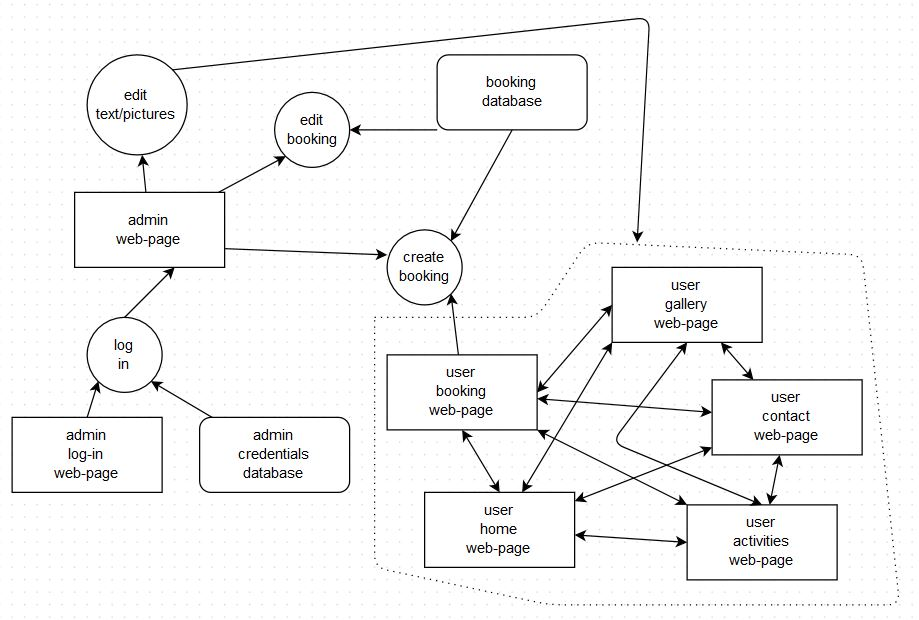
\includegraphics[scale=0.7]{usecasemodelV2.jpg}
\caption{Use Case model}
\end{figure}
Figur 1 illustrerer brugersiderne gallery, activities, home, contact og booking. Brugeren har gennem siden booking mulighed for at booke senge på hostelet. Bookingen bliver gemt i booking databasen. Den administrasive side kræver login. Der findes en database, der holder styr på logindetaljerne. Fra den administrative side kan kunden se og redigere i bookingerne samt teksten og billederne på de forskellige sider.\\
\subsection{c}

\begin{minipage}{\textwidth}

\captionof{table}{\textbf{Admin log-in}} \label{tab:title}
\begin{tabular}{| p{5cm} p{10cm} |}
\hline use-case-name & Admin log-in \\
\hline participating actors & administratoren \\
\hline flow of events & \begin{enumerate}
\item administratoren intaster sit log-in på admin log-in siden og trykker på log-in knappen
\item admindatabasen bliver spurgt om de indsendte oplysninger er rigtige.
\item hvis der findes et match, bliver man videreført til admin-siden. Hvis ikke får man en fejlmeddelelse.
\end{enumerate} \\
\hline Entry conditions & ingen \\
\hline Exit conditions & ingen \\
\hline
\end{tabular}

\end{minipage}

\bigskip

\begin{minipage}{\textwidth}

\captionof{table}{\textbf{Admin slet booking}} \label{tab:title}
\begin{tabular}{| p{5cm} p{10cm} |}
\hline use-case-name & Admin slet booking \\
\hline participating actors & administratoren \\
\hline flow of events & \begin{enumerate}
\item administratoren trykker på slet knappen i tabellen ud for bookingen 
\item ændringen bliver sendt til databasen og bookingen slettes
\item tabellen opdateres og bookingen er slettet og vises ikke mere
\end{enumerate} \\
\hline Entry conditions & admin log-in \\
\hline Exit conditions & ingen \\
\hline
\end{tabular}

\end{minipage}
	
\bigskip

\begin{minipage}{\textwidth}

\captionof{table}{\textbf{kunde booking}} \label{tab:title}
\begin{tabular}{| p{5cm} p{10cm} |}
\hline use-case-name & kunde booking \\
\hline participating actors & kunden \\
\hline flow of events & \begin{enumerate}
\item kunden indtaster sine ønskede booking datoer og kontaktinformationer 
\item kunden trykker på booking knappen og booking informationerne bliver tjekket for at verificere om bookingen ikke overlapper med andre bookinger
\item hvis der ikke er nogen overlab, bliver bookingen oprettet og kunden bliver videresendt til "home" siden. Hvis der er overlab får kunden en fejlmeddelelse
\end{enumerate} \\
\hline Entry conditions & at kunden befinder sig på bookingsiden \\
\hline Exit conditions & ingen \\
\hline
\end{tabular}

\end{minipage}	
	
\subsection{d}
\begin{figure}[H]
\centering
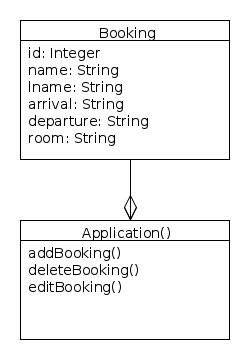
\includegraphics[scale=0.6]{BookingSystem.jpg}
\caption{Booking system - UML}
\end{figure}
Figur 2 illustrerer et klassediagram over vores bookingsystem. Application() tilføjer, redigerer og sletter bookinger fra bookingdatabasen. Booking definerer hvilke parametre en booking skal indeholde.
\subsection{e}

\begin{minipage}{\textwidth}

\captionof{table}{\textbf{Boundary}} \label{tab:title}
\begin{tabular}{| p{5cm} | p{10cm} |}
\hline Admin log-in side & web-siden for administratoren som benyttes til at verificere at personen er administrator \\
\hline kunde booking web-side & her har kunden adgang til at oprette en booking samt navigering til de andre kunde sider \\
\hline kunde "home" web-side & her kan kunden navigere til de andre sider \\
\hline kunde galleri web-side & her kan kunden navigere til de andre sider \\
\hline kunde kontakt web-side & her kan kunden navigere til de andre sider \\
\hline kunde aktiviteter web-side & her kan kunden navigere til de andre sider \\
\hline
\end{tabular}

\end{minipage}

\bigskip

\begin{minipage}{\textwidth}

\captionof{table}{\textbf{Control}} \label{tab:title}
\begin{tabular}{| p{5cm} | p{10cm} |}
\hline admin log-in \newline verificeringsknappen & facillitere forespørgslen mellem admin log-in siden og admin databasen, hvis personen er en admin, bliver vedkommende sendt videre til admin siden. hvis ikke, sker der ikke noget.\\
\hline opret booking knap & søger databasen for overlap i dato. Hvis der ikke er sådanne konflikter skabes en booking med de givne informationer i databasen, hvis der er en konflikt vises en passende fejlmeddelelse \\
\hline fjern booking knap & fjerner en oprettet booking fra databasen \\
\hline rediger web-sider & redigere kundesidernes indhold i forhold til billeder og tekst ( vi ved endnu ikke hvordan dette skal implementeres) \\
\hline "home" link & sender kunden til "home" web-page \\
\hline booking link & sender kunden til booking web-page \\
\hline galleri link & sender kunden til galleri web-page \\
\hline kontakt link & sender kunden til kontakt web-page \\
\hline aktiviteter link & sender kunden til aktiviteter web-page \\
\hline
\end{tabular}

\end{minipage}

\bigskip

\begin{minipage}{\textwidth}

\captionof{table}{\textbf{Entity}} \label{tab:title}
\begin{tabular}{| p{5cm} | p{10cm} |}
\hline Admin databasen & indeholder oplysninger om hvilke brugere der eksistere i systemet \\
\hline administrator siden & Her har administrator mulighed for at tilse aktuelle bookninger og rette i databasen \\
\hline booking database & indeholder alle bookinger på siden \\
\hline
\end{tabular}

\end{minipage}

\subsection{f}

\begin{figure}[H]
\centering
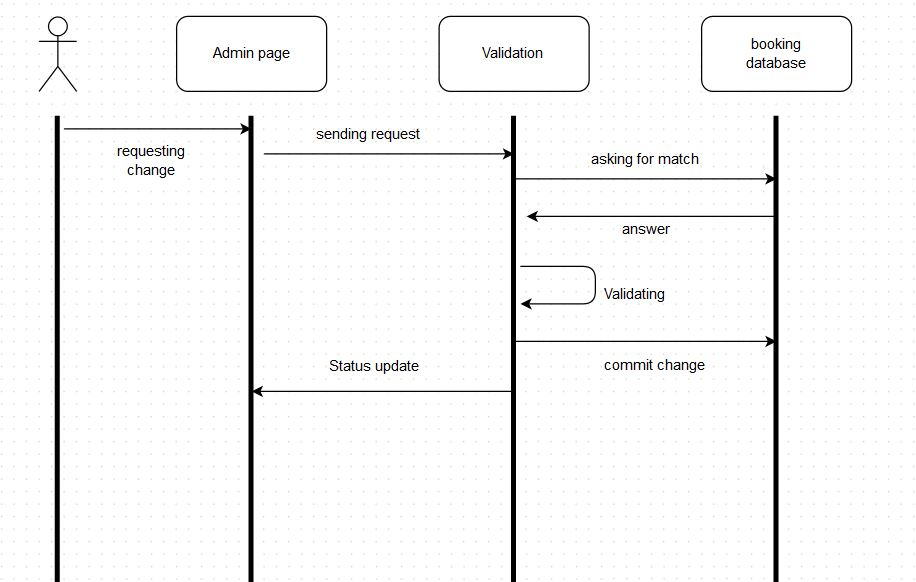
\includegraphics[scale=0.6]{adminInteraction.jpg}
\caption{Admin Interaction}
\end{figure}
Figur 4 illustrerer interaktionen mellem den administrative side og bookingdatabasen.\\
\begin{figure}[H]
\centering
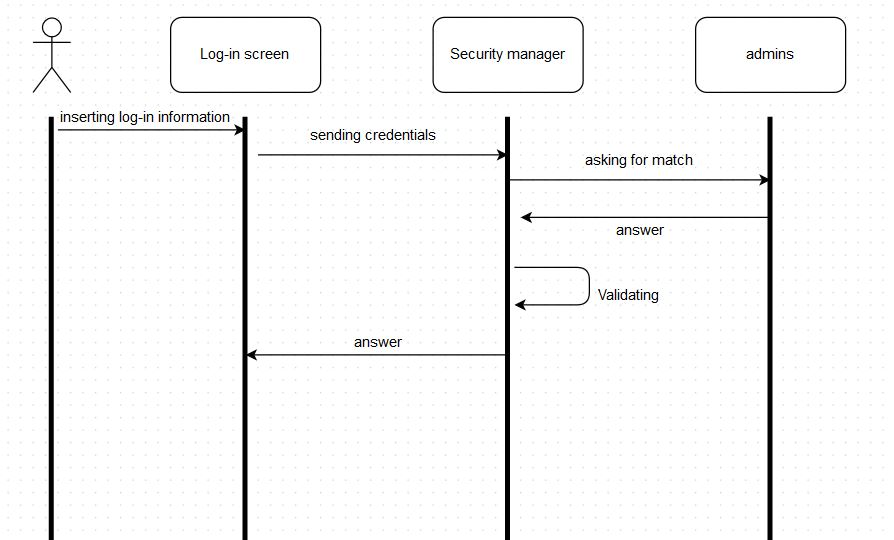
\includegraphics[scale=0.6]{adminLog-in.jpg}
\caption{Admin log-in}
\end{figure}
Figur 5 illusterer valideringprocessen ved login på den administrative side.\\
\begin{figure}[H]
\centering
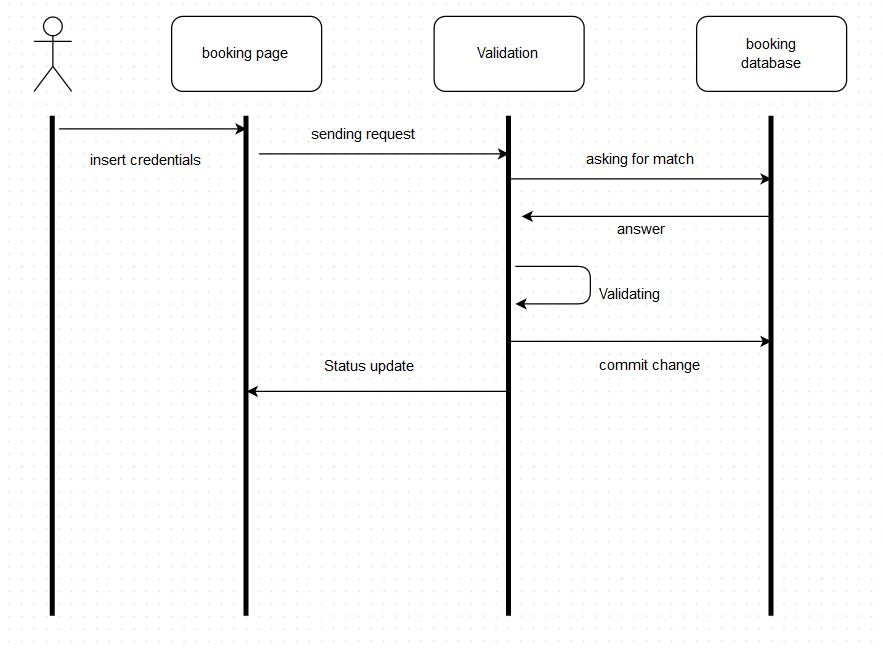
\includegraphics[scale=0.6]{customerLog-in.jpg}
\caption{Customer Interaction}
\end{figure}
Firgur 6 illustrerer processen når en bruger forsøger at oprette en booking.
\newpage
\section{Systemdesign sammenfatning}
\textbf{Systemet som det er nu:}
Vi har benyttet Play! frameworket til at lave en meget fin prototype at systemet.
Det er nu muligt at navigere mellem alle de forskellige sider, på hjemmesiden. Vi har fået implementeret en billede-slider på siden \textit{Gallery}, som præsenterer billeder af stedet i et diasshow. På siden \textit{Contact} har vi implementeret et google-maps kort, der viser hostelets beliggenhed. Bookingsystemet er også blevet konstrueret, og det er nu muligt at tilføje en booking fra bruger-siden, samt tilføje og slette bookinger fra admin-siden. Bookingerne gemmes i en database.    

\textbf{De væsentligste mangler:}
Vi mangler en funktion der gør det muligt for administratoren at ændre en booking. Desuden mangler vi stadig at lave et login-system til admin-siden.\\
Vi skal også gøre det muligt for kunden, selv at bestemme hvilke billeder der fremvises samt redigere i teksten på de forskellige sider. Endeligt mangler vi at koble bookingsystemet til et betalingssystem.
\section{Program- og systemtest}
Indtil videre har vi kun testet vores system visuelt, og alt virker som vi ønsker. Vi har endnu ikke sat begrænsninger på bookingsystemet, sådan at to bookinger ikke overlapper hinanden. Planen er at lave en test-klasse, der kan teste bookingsystemet med Junit.
\section{Brugergrænseflade og interaktonsdesign}

\subsection{eksempler på brugergrænseflade}
\begin{verbatim}
i figur 6 ses vors booking side hvor man kan oprette en booking. 
Det foreløbige design er således at der udover den oblikatoriske meny-bar 
også er fire tekstfelter, en "drop-down" meny og en knap.
Disse felter skal indsamle det data der bliver til en oprettet booking 
( indholdet af en booking er ikke færdigt endnu, 
der vil altså være andre/anderledes parametre i slutproduktet)  
\end{verbatim}
\begin{figure}[H]
\centering
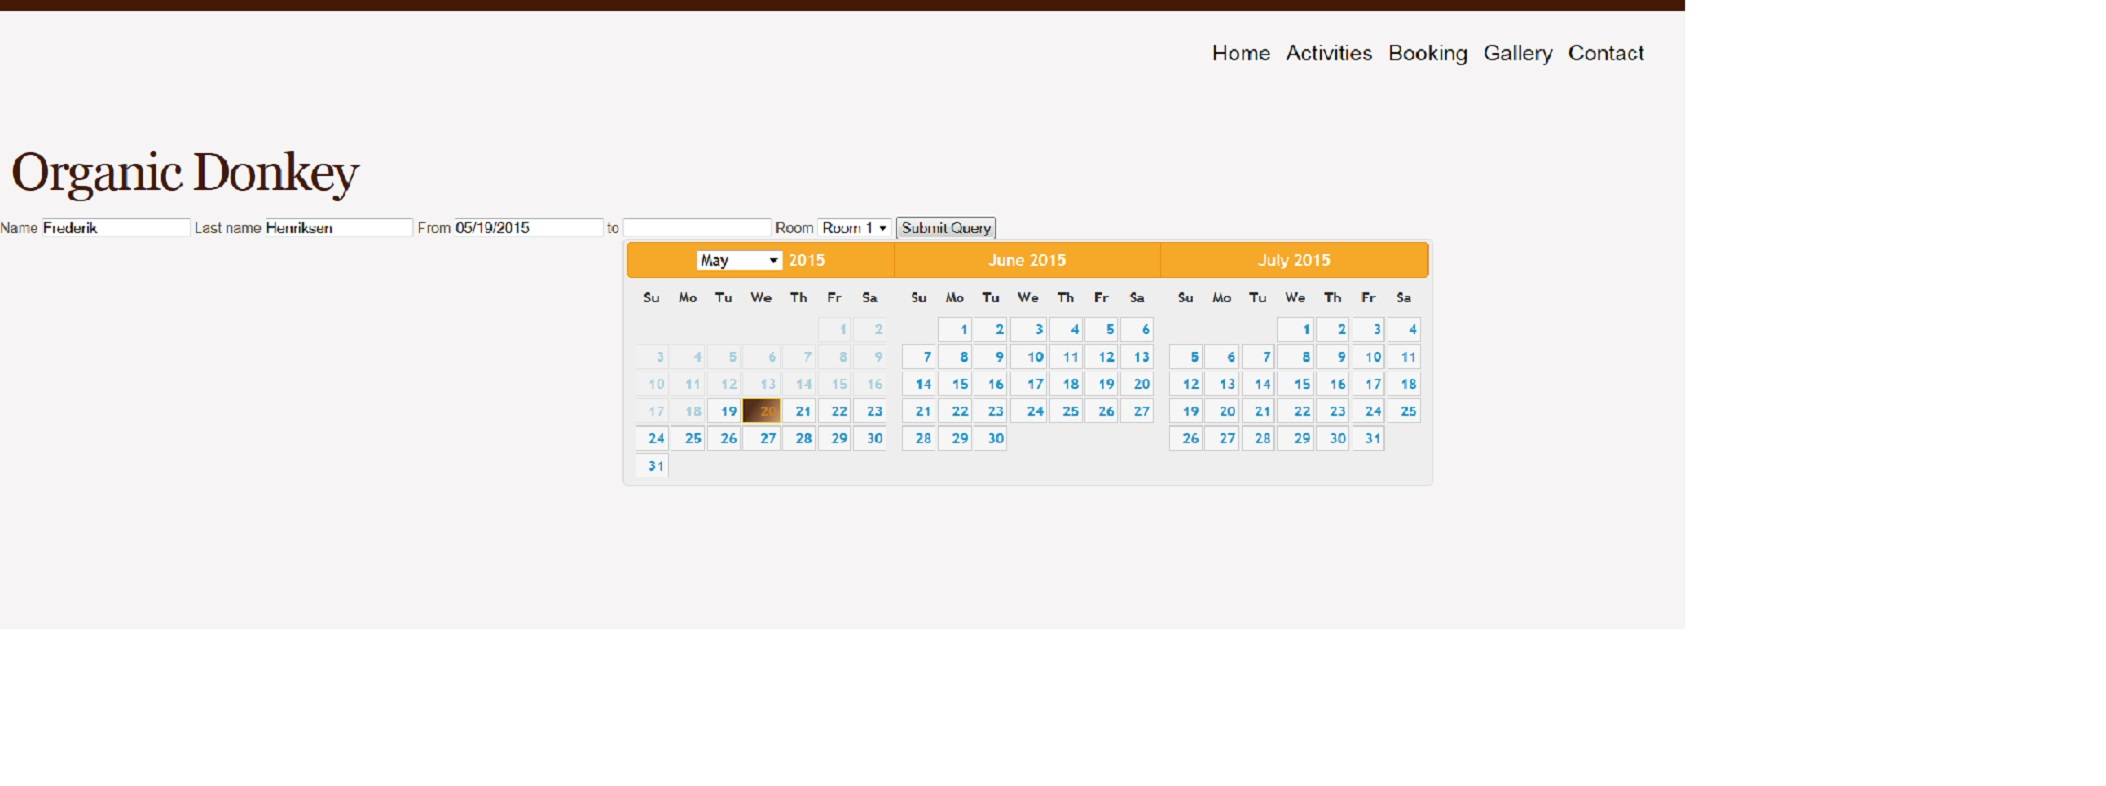
\includegraphics[scale=0.5] {brugergransefladebilled1.jpg}
\caption{opretter en booking}
her ses en bookning der er ved at blive lavet, hvor brugeren er ved at vælge dato
\end{figure}
\begin{verbatim}
I fugur 7 ses det layout som går igen på de fleste sider,
 med overskrift, meny-bar og teskt.
\end{verbatim}
\begin{figure}[H]
\centering
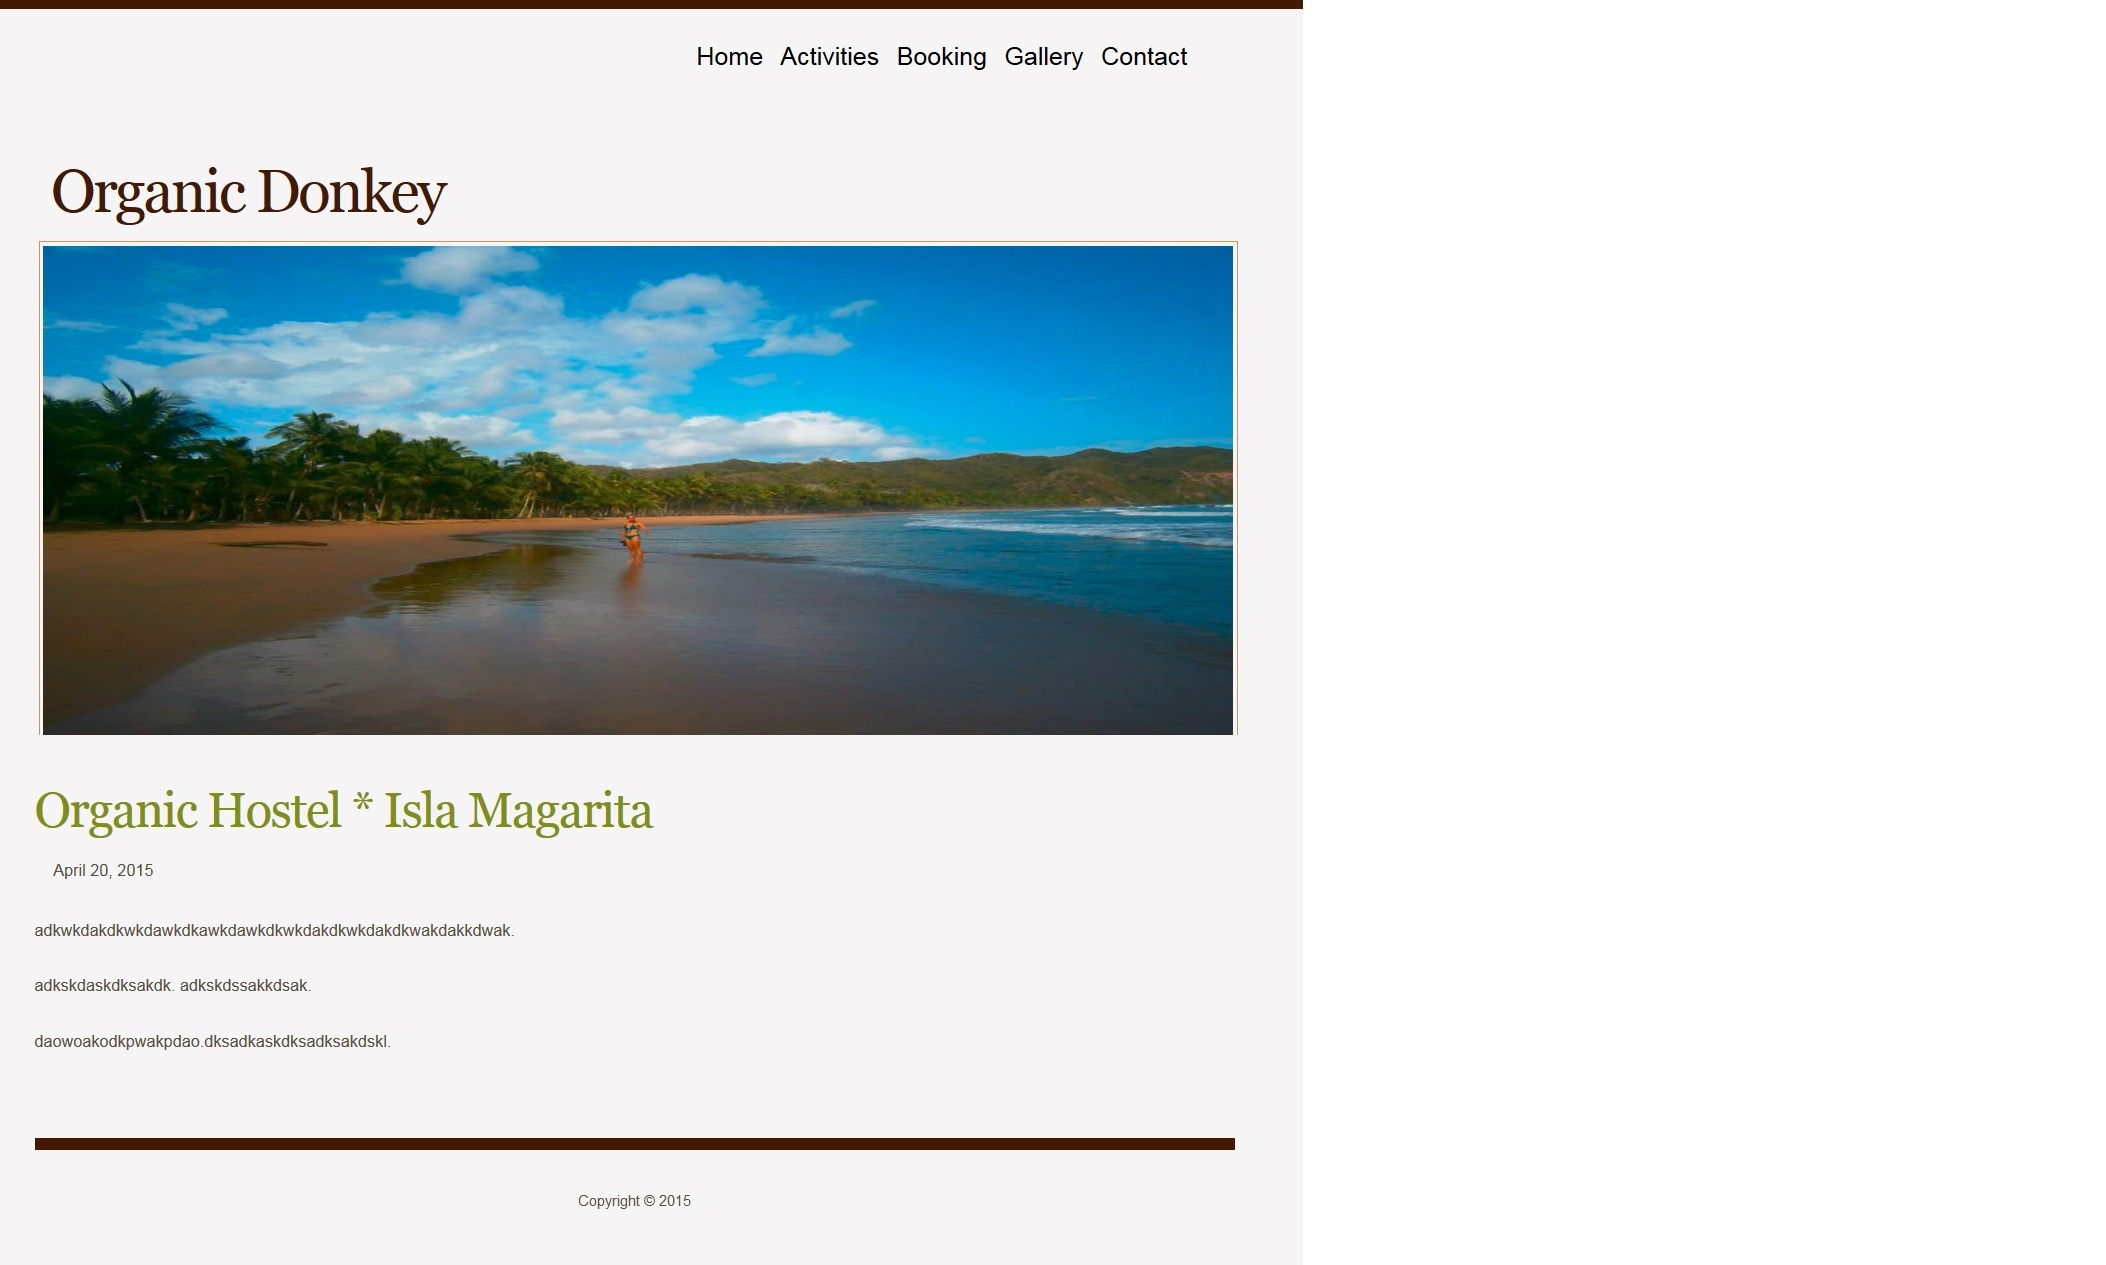
\includegraphics[scale=0.6] {brugergransefladebilled2.jpg}
\caption{index siden}
her ses vores sides forside 
\end{figure}
\begin{verbatim}
I figur 8 ses den forløbige admin side hvor administrator har overblikket
over bookinger(admin kan søge og slette bookinger) 
\end{verbatim}
\begin{figure}[H]
\centering
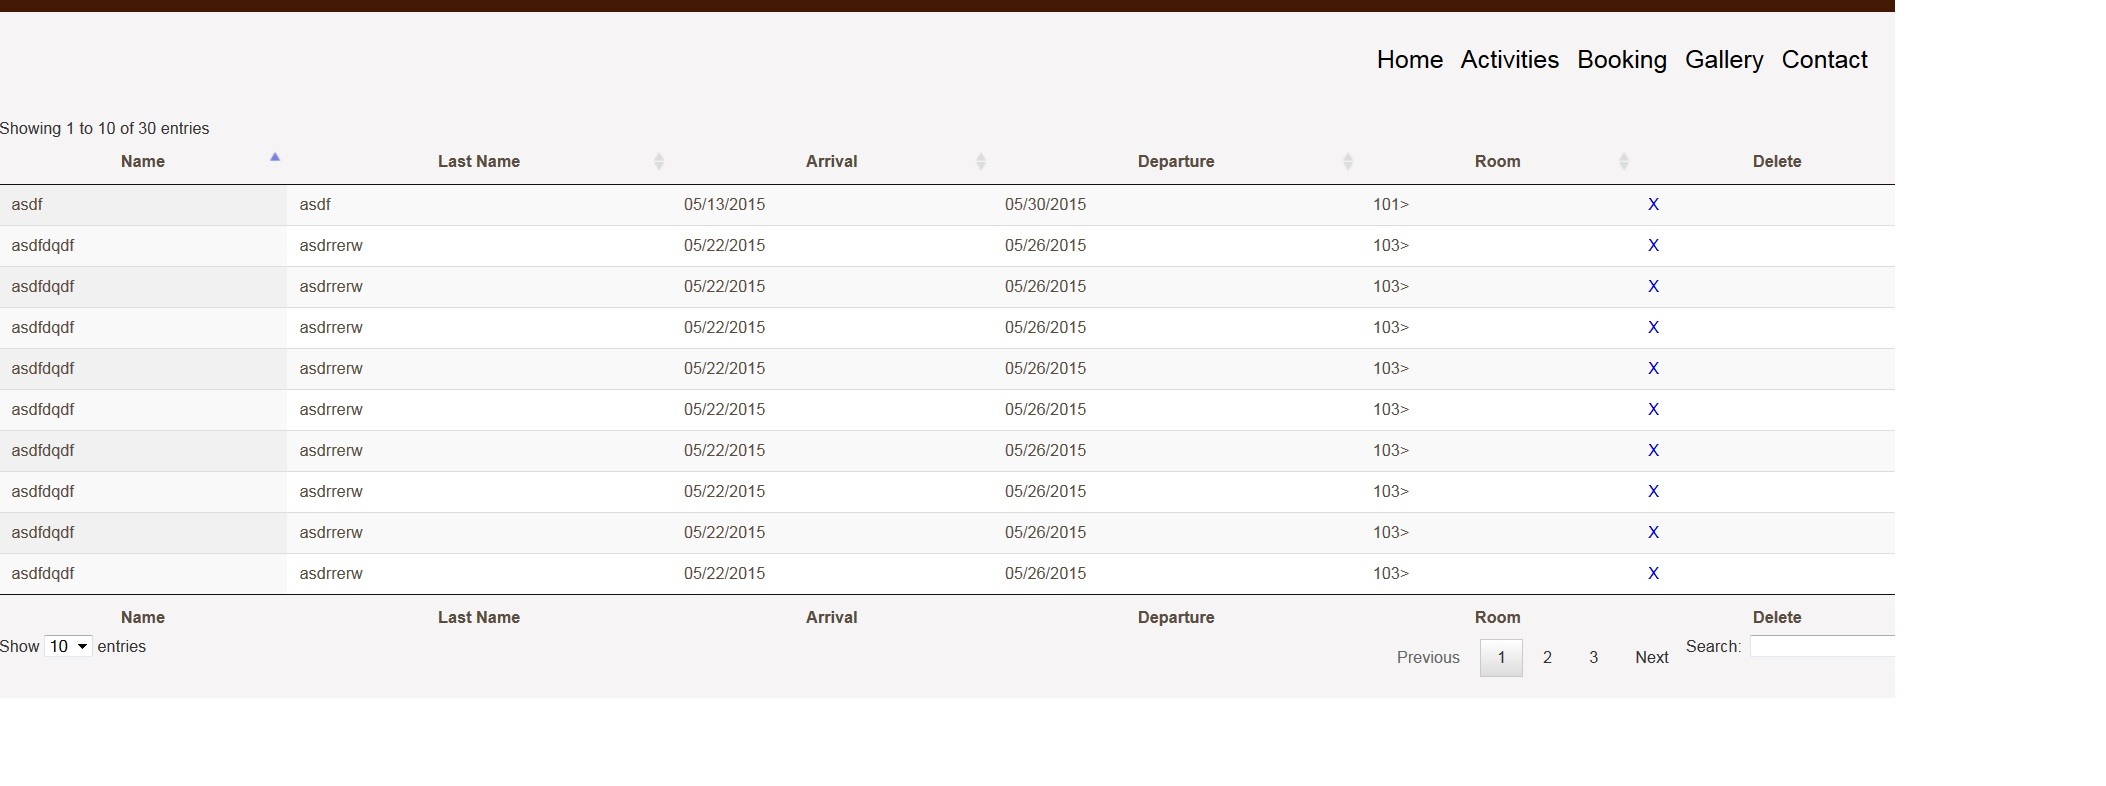
\includegraphics[scale=0.4] {brugergransefladebilled3.jpg}
\caption{oprettede bookinger}
her ses admin siden hvor admin kan se og slette bookinger
\end{figure}

\subsection{dynamikken i brugerinteraktion}
\begin{verbatim}
i figur 9 ses rutediagrammet over 
hvordan brugere af siden kan bevæge sig imellem de forskellige views. 
Dette er for kundens vedkommende gjordt ved at bruge meny-baren.
Det er for admin gjordt ved at logge ind.
\end{verbatim}
\begin{figure}[H]
\centering
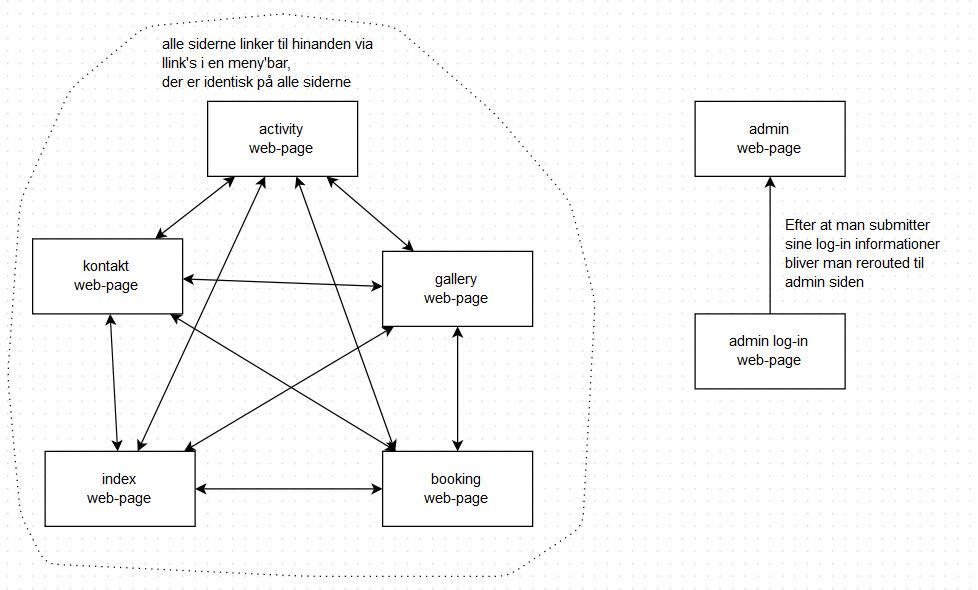
\includegraphics[scale=0.6] {flowchart.jpg}
\caption{flowchart over siden}
her ses rutediagrammet som siden fungere på nuværende tidspunkt
\end{figure}

\subsection{audio-visual præsentation}
Den forløbige viden : https://youtu.be/CF55ggqy9M8
\section{Projektsamarbejdet}
Internt i gruppen arbejder vi godt sammen. For nogle uger siden besluttede vi os for at sætte mandag og torsdag af til at arbejde på projektet. Siden da er vi nået rigtig langt med systemet. 

Vi har indtil videre haft tre møder med kunden. Møderne foregår over Skype, da kunden bor i Venezuela. På trods af at afstanden kan være upraktisk, er kunden fleksibel med dato for møder, da vi blot mødes over Skype.

Under møderne tager vi referat i form af stikord, og dokumenterer de aftalte ændringer i projektaftalen og projektplanen, i rapporten. 

Under første møde d. 19. februar 2015 fik vi lavet en projektaftale med kunden.\\
Under andet møde d. 10. marts 2015 snakkede vi detaljer ift. bookingsystemet.\\
Under tredje møde d. 15. april 2015 snakkede vi om valg af betalingssystem, samt om hvilke dele af projektet kunden helst så os nedprioritere i tilfælde af tidspres.

Vi har endnu ikke en fast dato for næste møde, da kunden som sagt er fleksibel, og vi derfor kan kontakte hende, når vi har brug for at diskutere projektet.
\newpage
\section{Litteraturreview}
\subsection{Review af The M.A.D experience, Christensen et al. (1998)}
The M.A.D experience er en artikel omhandlende en research gruppe fra Århus universitet, der  ingår et samarbejde med et stort glabalt shippingfirma om at lave en prototype til et kundeservicesystem. 
Arktiklen handler, om hvordan gruppen får designet og implementeret en rigtig god prototype, der endda overgår shipping firmaets forventninger. Dette uden at gruppen havde nogen som helst form for ekpertise inden for shippingområdet.
Artiklen diskuterer, hvilke delelementer der spillede en rolle for denne succesfulde udføring af projektet.
Gruppemedlemmerne havde tre forskellige roller: en etnograf, en participatorisk designer og seks objektorienterede designere. 

Etnografen står for at udforme et design, der sørger for, at systemet relaterer til det miljø, projektet omhandler. Han identificerer problemløsningsområdet men ikke selve designløsningerne.

Den participatoriske designer arbejder med vigigheden i at involvere potentielle brugere af systemet i den kreative designprocess. Dette gøres både ud fra et moralsk og et praktisk grundlag, da det er rimeligt at lade de, som i sidste ende skal bruge systemet, være med til at tage beslutninger, og at disse personer samtidig er de mest praktiske forsøgspersoner at have med ind over projektet. 
Den participatoriske designer går op i at afholde workshops for forskellige mennesker, der har en eller anden tilknytning til projektet, for derefter at indrette systemdesignet udfra den konstruktive kritik de modtager under disse workshops.

De objektorienterede designere integrerer analyserne og designet fra etnografen og den participatoriske designer i det endelige design og implementering at systemet.

Udover disse tre elementer kommenterer artiklen på, at det er vigtigt, at man kommer igang med programmeringen så tidligt som muligt, bl.a. så man har noget at vise frem og få feedback på fra kunden og brugerne. Men også fordi at det i deres projekt, som også diskuteret i A Rational Design Process \footnote{Parnas and Clements 1986: A Rational Design Process: How and Why to Fake It }, ikke stod klart fra start af, præcis hvordan systemet skulle udformes. 
De fandt, at man altid ville ende op med et andet design end den initielle design struktur, blandt andet på grund af den feedback de fik fra kunden og brugerne. 

Det konkluderes, at et succesfuldt projekt kan opnås ved at have fokus på analyse af det miljø og det praktiske, som systemet omhandler, og skal henvende sig til. Disse elementer skal optræde som en integreret del af implementeringen af projektet.
\subsection{No silver bullet}
No Silver Bullet – Essence And Accidents in Software Engineering handler om software udvikling og dets vanskeligheder (essentiel og utilsigtet) og løsningerne på problemerne. 

Han undersøger arten af programfejl, og egenskaberne af de løsninger som han selv kalder silver bullets. 

Brooks mener, at den sværeste del af software udvikling er de arkitektoniske opgaver som specifikation, design og test af konstruktionen.

Vanskelighederne er delt op i essentielle og utilsigtet typer. De essentielle problemer er medfødte  til software. En kompleks og præcis abstrakt konstruktion afledt af datasæt, dataelementer, algoritmer og funktioner. De utilsigtet problemer er de problemer der opstår, når en udvikler er i gang med at udvikle softwaren men er ikke medfødte i selve softwaren.

Brooks opstiller de essentielle vanskeligheder som kompleksitet, overenstemmelse, foranderlig og usynlighed. De uvæsentlig problemer er ikke opstillet så klart.

Tre løsninger på utilsigtet  problemer bliver diskuteret. Det er høj niveau programmerings sprog, multiprogrammering og forenet udviklings miljøer. Det største gennembrud for produktiviteten, pålideligheden og enkelhed af de tre løsnings forslag er høj niveau sprog. Høj niveau sprog giver stærke fælles konstruktioner til programmøren og reducere et niveau af software kompleksitet.

I vores projekt hvor vi skal udvikle en hjemmeside med et booking system til nogle sommerhuse i Venezuela. Har vi også benyttet os af et høj niveau sprog som gør udvikling for vores projekt en del lettere og er med til at optimerer vores program. OOSE bogen anbefaler også brug af høj niveau sprog til udvikling, da der er mange tilgængelig pakker der kan hjælpe til udviklingen.

For at samle vores projekt et sted der gør det let tilgængeligt for os alle og gør det muligt for os at udvikle på dele af programmet er github.
\end{document}